\begin{figure}[htbp]
\centering
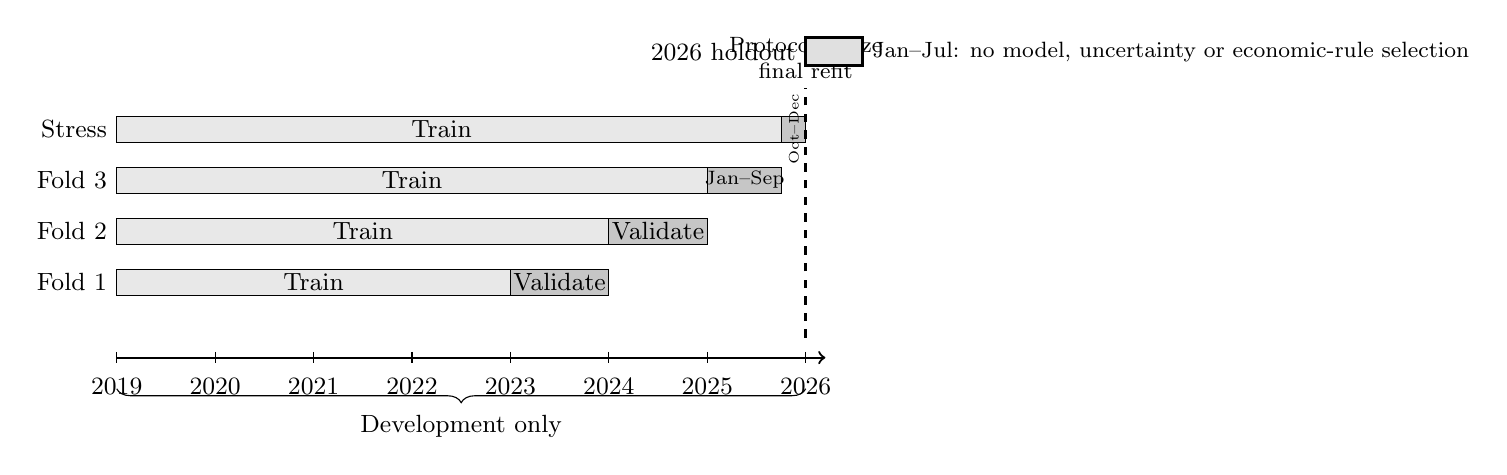
\begin{tikzpicture}[x=1.25cm,y=0.72cm,font=\small]
% year axis
\draw[->,thick] (0,0) -- (7.2,0);
\foreach \x/\lab in {0/2019,1/2020,2/2021,3/2022,4/2023,5/2024,6/2025,7/2026}
  \draw (\x,0.1)--(\x,-0.1) node[below=2pt] {\lab};

% Fold bars
\draw[fill=gray!18,draw] (0,1.1) rectangle (4,1.55);
\draw[fill=gray!45,draw] (4,1.1) rectangle (5,1.55);
\node[left] at (0,1.33) {Fold 1};
\node at (2,1.33) {Train};
\node at (4.5,1.33) {Validate};

\draw[fill=gray!18,draw] (0,2.0) rectangle (5,2.45);
\draw[fill=gray!45,draw] (5,2.0) rectangle (6,2.45);
\node[left] at (0,2.23) {Fold 2};
\node at (2.5,2.23) {Train};
\node at (5.5,2.23) {Validate};

\draw[fill=gray!18,draw] (0,2.9) rectangle (6,3.35);
\draw[fill=gray!45,draw] (6,2.9) rectangle (6.75,3.35);
\node[left] at (0,3.13) {Fold 3};
\node at (3,3.13) {Train};
\node at (6.38,3.13) {\scriptsize Jan--Sep};

\draw[fill=gray!18,draw] (0,3.8) rectangle (6.75,4.25);
\draw[fill=gray!45,draw] (6.75,3.8) rectangle (7,4.25);
\node[left] at (0,4.03) {Stress};
\node at (3.3,4.03) {Train};
\node[rotate=90] at (6.88,4.03) {\tiny Oct--Dec};

% freeze and holdout
\draw[very thick,dashed] (7,0.35) -- (7,4.75);
\node[above,align=center,font=\footnotesize] at (7,4.75) {Protocol freeze\\final refit};
\draw[fill=black!12,draw,very thick] (7,5.15) rectangle (7.58,5.65);
\node[left] at (7,5.4) {2026 holdout};
\node[right,font=\footnotesize] at (7.58,5.4) {Jan--Jul: no model, uncertainty or economic-rule selection};

\draw[decorate,decoration={brace,mirror,amplitude=5pt}] (0,-0.55) -- (7,-0.55)
 node[midway,below=6pt] {Development only};
\end{tikzpicture}
\caption{Chronological development and holdout design. Model and uncertainty choices are made using 2019--2025 only. The protocol is frozen before the January--July 2026 first-look holdout is evaluated.}
\label{fig:timeline}
\end{figure}
